\documentclass[a4paper,11pt]{article}
\usepackage{amsmath,amsthm,amsfonts,amssymb,amscd,amstext,vmargin,graphics,graphicx,tabularx,multicol} 
\usepackage[francais]{babel}
\usepackage[utf8]{inputenc}  
\usepackage[T1]{fontenc} 
\usepackage{pstricks-add,tikz,tkz-tab,variations}
\usepackage[autolanguage,np]{numprint} 
\usepackage{color}
\usepackage{ulem}

\setmarginsrb{1.5cm}{0.5cm}{1cm}{0.5cm}{0cm}{0cm}{0cm}{0cm} %Gauche, haut, droite, haut
\newcounter{numexo}
\newcommand{\exo}[1]{\stepcounter{numexo}\noindent{\bf Exercice~\thenumexo} : \marginpar{\hfill /#1}}
\reversemarginpar


\newcounter{enumtabi}
\newcounter{enumtaba}
\newcommand{\q}{\stepcounter{enumtabi} \theenumtabi.  }
\newcommand{\qa}{\stepcounter{enumtaba} (\alph{enumtaba}) }
\newcommand{\initq}{\setcounter{enumtabi}{0}}
\newcommand{\initqa}{\setcounter{enumtaba}{0}}

\newcommand{\be}{\begin{enumerate}}
\newcommand{\ee}{\end{enumerate}}
\newcommand{\bi}{\begin{itemize}}
\newcommand{\ei}{\end{itemize}}
\newcommand{\bp}{\begin{pspicture*}}
\newcommand{\ep}{\end{pspicture*}}
\newcommand{\bt}{\begin{tabular}}
\newcommand{\et}{\end{tabular}}
\renewcommand{\tabularxcolumn}[1]{>{\centering}m{#1}} %(colonne m{} centrée, au lieu de p par défault) 
\newcommand{\tnl}{\tabularnewline}

\newcommand{\trait}{\noindent \rule{\linewidth}{0.2mm}}
\newcommand{\hs}[1]{\hspace{#1}}
\newcommand{\vs}[1]{\vspace{#1}}

\newcommand{\N}{\mathbb{N}}
\newcommand{\Z}{\mathbb{Z}}
\newcommand{\R}{\mathbb{R}}
\newcommand{\C}{\mathbb{C}}
\newcommand{\Dcal}{\mathcal{D}}
\newcommand{\Ccal}{\mathcal{C}}
\newcommand{\mc}{\mathcal}

\newcommand{\vect}[1]{\overrightarrow{#1}}
\newcommand{\ds}{\displaystyle}
\newcommand{\eq}{\quad \Leftrightarrow \quad}
\newcommand{\vecti}{\vec{\imath}}
\newcommand{\vectj}{\vec{\jmath}}
\newcommand{\Oij}{(O;\vec{\imath}, \vec{\jmath})}
\newcommand{\OIJ}{(O;I,J)}

\newcommand{\bmul}[1]{\begin{multicols}{#1}}
\newcommand{\emul}{\end{multicols}}

\newcommand{\reponse}[1][1]{%
\multido{}{#1}{\makebox[\linewidth]{\rule[0pt]{0pt}{20pt}\dotfill}
}}

\newcommand{\titre}[5] 
% #1: titre #2: haut gauche #3: bas gauche #4: haut droite #5: bas droite
{
\noindent #2 \hfill #4 \\
#3 \hfill #5

\vspace{-1.6cm}

\begin{center}\rule{6cm}{0.5mm}\end{center}
\vspace{0.2cm}
\begin{center}{\large{\textbf{#1}}}\end{center}
\begin{center}\rule{6cm}{0.5mm}\end{center}
}



\begin{document}
\pagestyle{empty}
\titre{Interrogation: Bases de la géométrie}{Nom :}{Prénom :}{Classe}{Date}



\vspace*{1cm}

\exo{5} Questions de cours\\

\q Donner la définition d'un point.\\
\textcolor{red}{Un point du plan est un lieu , un endroit qui n’a ni longueur ni épaisseur .Il existe partout des points, qui ne sont
pas nécessairement marqués ou encore moins nommés.}\\

\q Donner la définition d'un segment.\\
\textcolor{red}{Un segment est une ligne droite limitée des deux côtés par ses extrémités.}\\

\q Donner la définition d'une demi-droite.\\
\textcolor{red}{Une demi-droite est une ligne droite limitée d’un côté par un point qu'on appelle "origine" et illimitée de
l'autre côté.}\\

\q Trouver les erreurs dans le tracé de la figure ci-dessous et \textbf{corriger-les}.\\
\newrgbcolor{qqttzz}{0 0.2 0.6}
\newrgbcolor{qqzzqq}{0 0.6 0}
\psset{xunit=1.0cm,yunit=1.0cm,algebraic=true,dotstyle=o,dotsize=3pt 0,linewidth=0.8pt,arrowsize=3pt 2,arrowinset=0.25}
\begin{pspicture*}(0.24,-1.74)(12.56,4.62)
\psplot[linecolor=red]{0.24}{12.56}{(--19.55-0.88*x)/5.94}
\psplot[linecolor=qqttzz]{2.1}{12.56}{(--32.25-3.58*x)/8.3}
\psline[linecolor=qqzzqq](8.04,2.1)(10.4,-0.6)
\begin{scriptsize}
\psdots[dotstyle=x,linecolor=blue](2.1,2.98)
\rput[bl](2.18,3.1){\blue{$R$}}
\psdots[dotstyle=x,linecolor=blue](8.04,2.1)
\rput[bl](8.12,2.22){\blue{$I$}}
\psdots[dotstyle=x,linecolor=blue](10.4,-0.6)
\rput[bl](10.48,-0.48){\blue{$G$}}
\end{scriptsize}
\end{pspicture*}

\q Décrire la figure ci-dessus.\\
\textcolor{red}{Sur la figure ci-dessus, on peut y voir une droite (RI), un segment [IG] et une demi-droite [RG).}\\


\exo{1,5}

\bmul{2}

\vspace*{1cm}

\noindent Tracer en vert le segment d'extrémités D et C. \\
Tracer en rouge la droite passant par A et C.\\
Tracer en bleu la demi-droite d'origine D passant par B.

\columnbreak

\begin{flushleft}
\includegraphics[scale=1]{correctionexo.eps} 
\end{flushleft}

\emul

\newpage

\exo{1,5}

\begin{flushleft}
\includegraphics[scale=1]{correction2.eps} 
\end{flushleft}

\exo{2} Compléter les expressions suivantes avec les symboles "$\in$" ou "$\notin$"\\

\bmul{2}

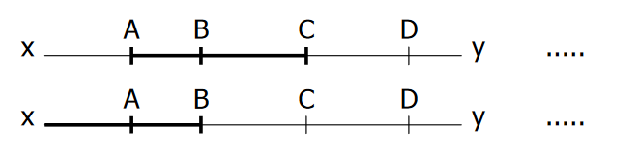
\includegraphics[scale=1]{exointerro3.eps} 

\columnbreak

\vspace*{1cm}
\bmul{2}

B \textcolor{red}{$\in$} [AH)\\

F  \textcolor{red}{$\notin$} (DE)

\columnbreak
C \textcolor{red}{$\notin$} [AE]\\

H  \textcolor{red}{$\notin$} [BA)

\emul


\emul

\end{document}
